%============================ Project Managenent Document ================================
% define document class
\documentclass[
	a4paper               % paper format
%	,10.5pt               % fontsize
%	,BCOR=18mm            % Binding correction
	,bibliography=totoc   % If enabled add bibliography to TOC
	,listof=totoc         % If enabled add lists to TOC
%	,bilingual
	,monolingual
	twoside=false,
]{bfhthesis}              % KOMA-script report

\setcounter{secnumdepth}{4}

\PassOptionsToPackage{hyphens}{url}\usepackage[
	hidelinks,
	pdfusetitle,
]{hyperref}
\usepackage{tikzducks}
\usepackage{amsmath}
\usepackage{listings}

\LoadBFHModule{boxes}

\colorlet{punct}{red!60!black}
\definecolor{background}{HTML}{EEEEEE}
\definecolor{delim}{RGB}{20,105,176}
\colorlet{numb}{magenta!60!black}

\lstdefinelanguage{json}{
    basicstyle=\normalfont\ttfamily,
    numbers=left,
    numberstyle=\scriptsize,
    stepnumber=1,
    numbersep=8pt,
    showstringspaces=false,
    breaklines=true,
    frame=lines,
	postbreak=\mbox{\textcolor{red}{$\hookrightarrow$}\space},
    backgroundcolor=\color{background},
    literate=
      {:}{{{\color{punct}{:}}}}{1}
      {,}{{{\color{punct}{,}}}}{1}
      {\{}{{{\color{delim}{\{}}}}{1}
      {\}}{{{\color{delim}{\}}}}}{1}
      {[}{{{\color{delim}{[}}}}{1}
      {]}{{{\color{delim}{]}}}}{1},
}

\lstdefinelanguage{canon}{
    basicstyle=\normalfont\ttfamily,
    numbers=left,
    numberstyle=\scriptsize,
    stepnumber=1,
    numbersep=8pt,
    showstringspaces=false,
    breaklines=true,
    frame=lines,
    backgroundcolor=\color{background},
	postbreak=\mbox{\textcolor{red}{$\hookrightarrow$}\space},
}

\hyphenation{ve-ri-fi-ca-ti-on}

\begin{document}

\frontmatter

\title{Bachelor's Thesis}
\subtitle{Unlinkability of Verfiable Credentials in a practical approach
: Project Management Document}
\author{Joël Gabriel Robles Gasser}
\institution{Bern University of Applied Sciences}
\department{Engineering and Computer Science}
\institute{Computer Science}
\version{0.1}
\advisor{Prof. Dr. Annett Laube \and Prof. Dr. Reto Koenig}
\expert{Dr. Andreas Spichiger}
\degreeprogram{Bachelor of Science in Computer Science}

%----------------  BFH tile page   -----------------------------------------
\maketitle

\addchap{Abstract}
Here an abstract might be placed.


%------------ TABLEOFCONTENTS ----------------
\tableofcontents

%------------ START MAIN PART ----------------
\mainmatter

\chapter{Introduction}
Self-sovereign Identity (SSI)\cite{self-sovereign-identity} is a concept where individuals can control their digital identity and what data is shared with whom.
In the real world physical credentials like an ID or a driver's license are used, which makes selectively disclosing information hard, as there is more information on the credentials as there is needed in one presentation.
If we digitalize these credentials, we create the option for individuals to selectively disclose information. 
Verifiable credentials (VCs)\cite{verifiable-credentials} are a type of digital credentials that can be used to represent physical credentials.
These digital credentials support multiple signing themes, one of which is the BBS Signature scheme (BBS)\cite{bbs-signature-scheme}.
This signature scheme is based on the trust triangle seen in figure \ref{fig:trusttringle}, where there are three involved parties.

\begin{figure}[h]
	\centering
	\includegraphics[width=4cm]{example-image-duck}
	\caption{The trust triangle}
	\label{fig:trusttringle}
\end{figure}

These parties are the issuer, holder and verifier.
The issuer supplies the credential to the holder, which stores it. The holder is then able to present it to a verifier, which checks its validity and content.
The verifier uses the signature to also check the authenticity and integrity of the supplied credential.
Besides signing, this signature scheme also supports proof creation, which enables unlinkability.
Unlinkability is the concept that there is no link between each credential presentation and different verifiers.
BBS also supports selective disclosure, to only disclose a subset of the information contained in the credential.\\

In this thesis we want to investigate the use of the BBS Signature Scheme in a real world scenario.
We assume that the BBS Signature scheme has no flaws, and the promoted unlinkability of the scheme holds in every situation.
We will also only use verifiable-credentials with data integrity, to not only protect the attributes of the credential (like the name, birthdate \dots) but to also protect the meta-data of the verifiable credential.
For the data integrity we will also use the BBS Signature Scheme.\\

The credentials need to send between the issuer and holder and between the holder and the verifier.
For this thesis we will only look at the messaging between the holder and the verifier and assume that the VC creation and transportation to the holder is secure.
For the presentation of the credentials there is an extension of VCs called a Verifiable-presentation (VP)\cite{verifiable-credentials}.
To present the VP we use OpenID-Connect for Verifiable-Presentations (OIDC4VP)\cite{oidc4vp}.
For OIDC4VP we assume that all communication is secured and encrypted.\\

\textit{Why not login?}
First of we would like to simply the process of a returning customer.
Think about how often you log in into Netflix, either with your email and password or with the cached login token.
It would be very unnecessary to present your VC each time you would like to watch a show, so we would like recognition.
To solve that problem we will look at Pseudonyms\cite{pseudonyms} in chapter \ref{chap:Pseudonyms}.\\

These Pseudonyms are used for a verifier to recognize already before seen individual.
This extension of the BBS Signature scheme should not break the unlinkability of the BBS proofs as they are only linkable between one verifier and the holder, but will still be analyzed.\\

Lastly we will look at the problem, where if we need to present two different VCs (like a driver's license and the vehicle registration document), how can we proof that both documents are owned by the same holder.
For that we will make use of link secrets\cite{linksecrets}, which is a secret value that only the holder knows.
% This value is supplied blinded to the issuer, meaning that is encoded in such a way that the issued cannot find out what the original value is.
% For the signer to be able to create a VC containing a blinded value, they would need to use Blind BBS Signatures\cite{bbs-signature-scheme}, which allows signing of such blinded values.
% With the blind signatures we also allow individuals to create their own credentials for their own needs, without needing to reveal the content of the credential, by using the ability to blind values.
% When a holder then presents two different credentials to a verifier, he can proof that both of those credentials are owned by him by proving the knowledge of the contents of the blinded link secrets.
In this thesis we want to analyse these concepts in conjunction with the BBS Signature scheme, to see if there is any data leakage or if the unlinkability provided by the BBS Signature Scheme will break.
For this we will investigate each concept step by step, based on their respective specifications, and implement them if needed.

\chapter{Goals}

\chapter{Risks}
In this chapter we define Risks that may happen in this thesis.

\section{Project Risks}

\subsection{VC}
\begin{itemize}
	\item Risk: There is the possibility that the structure of VCs breaks the unlinkability of BBS
	\item Solution: If that is the case, the stucture of VCs needs to be reworked so there is no linkability
	\item Possibility: Low
\end{itemize}

\subsection{OIDC4VP}
\begin{itemize}
	\item Risk: There is the possibility that the implementation of OIDC4VP leaks data
	\item Solution: If that is the case, the structure of the OIDC4VC protocol needs to be reworked so there are no more data leaks
	\item Possibility: Low
\end{itemize}

\subsection{OIDC4VP}
\begin{itemize}
	\item Risk: There is the possibility that the implementation of OIDC4VP leaks data
	\item Solution: If that is the case, the structure of the OIDC4VC protocol needs to be reworked so there are no more data leaks
	\item Possibility: Low
\end{itemize}
\begin{itemize}
	\item Risk: There is the possibility that the implementation of OIDC4VP breaks the unlinkability of BBS
	\item Solution: If that is the case, the structure of the OIDC4VP protocol needs to be reworked so there is no linkability
	\item Possibility: Medium
\end{itemize}

\subsection{Psuedonyms}
\begin{itemize}
	\item Risk: There is the possibility that the implementation of Pseudonyms breaks the unlinkability of BBS
	\item Solution: If that is the case, the structure of Pseudonyms needs to be reworked, so there is no linkability
	\item Possibility: Low
\end{itemize}

\subsection{Link Secrets}
\begin{itemize}
	\item Risk: There is the possibility that the implementation of Link Secrets breaks the unlinkability of BBS
	\item Solution: If that is the case, the implementation of the Link Secrets needs to be reworked, so there is no linkability
	\item Possibility: Medium
\end{itemize}
\begin{itemize}
	\item Risk: There is the possibility that the implementation of Link Secrets allows the holder of multiple VCs to Link the together on a different Secret
	\item Solution: If that is the case, the implementation of the Link Secrets needs to be reworked so that this is no longer possible
	\item Possibility: Low
\end{itemize}

\section{Environmental risks}

\subsection{Sickness}
\begin{itemize}
	\item Risk: There is a possibility that I may become sick
	\item Solution: If the sickness is less than 1 Week, there is a Buffer in the project plan at the end of the semester for that. If it's more than 1 Week, there is a chance that the Project would need to be moved to another semester
	\item Possibility: Medium
\end{itemize}

\subsection{Hardware}
\begin{itemize}
	\item Risk: There is a possibility that the Hardware used (Laptop) may break due to unknown reasons
	\item Solution: The Deliverables are backed u to GitHub and mirrored to the BFH-TI GitLab. There is also a Backup on other Hardware. There also Backup Hardware if the main Hardware would break
	\item Possibility: Low
\end{itemize}
\begin{itemize}
	\item Risk: There is the possibility that the Backups are not accessible
	\item Solution: For that case there is an also a Backup on different Devices
	\item Possibility: Low
\end{itemize}

\subsection{Project Plan/Ideas}
\begin{itemize}
	\item Risk: There is the possibility that the project plan is bad, so that the Planned time frames are to short
	\item Solution: In that case there is 1 week buffer at the end of the semester. If that is not enough time, then there needs to be an explanation in the documentation why that happened
	\item Possibility: Medium
\end{itemize}
\begin{itemize}
	\item Risk: There is the possibility that the expert of the project may bring new Ideas into the project
	\item Solution: If those ideas further the projects goals, they may be added to the project plan. In that case the Project plan needs to be reworked
	\item Possibility: Low
\end{itemize}

% \chapter{Recap of BLS12-381, BBS and Pairings}
% This chapter contains a quick recap about BBS and BLS12-381.
% The Mathematics of these topics are out of scope for this Thesis, so only the top level ideas will be discussed.

% \section{BLS12-381}
% \begin{figure}[h]
%     \centering
% 	\includegraphics[width=4cm]{example-image-duck}
% 	\caption{The BLS12-381 curve}
% 	\label{fig:bls12381}
% \end{figure}
% The Barreto-Lynn-Scott Curves \cite{pairing-friendly-curves} are a group of pairing friendly curves. 
% Specifically the BLS12-381 Curve is used in the BBS Signature Scheme \cite{bbs-signature-scheme}.
% The 12 in the name comes from the embedding degree, the 381 is the amount of bits necessary to represent a point on the curve.
% This Curve is defined as with the following equation $y^2 = x^3 + 4$, where x and y are coordinates on the Field $F_p$.

% \subsection{Field Extensions}
% $G_1$ is the largest is the largest prime order subgroup of the BLS curve.
% For the Pairings discussed in section \ref{sec:pairing} we need multiple points on curves as inputs.
% Besides a point on $G_1$ we also need a point on $G_2$.
% This $G_2$ is an Extension of the Field $F_p$ into the Field $F_{p^2}$.
% This alters the curve equation a bit to $y^2 = x^3 + 4(u + 1)$ where x and y are no longer coordinates but are polynoms of the second order.
% Both $G_1$ and $G_2$ are additive Groups.
% For the Pairings we also need a third Group, this time in the Field $F_{p^{12}}$.
% This is Group is a multiplicative group called $G_T$ in section \ref{sec:pairing}, where x and y are polynoms of the $12^{th}$ order.
% With this we now know all the necessary groups for \ref{sec:bbs}.
% The Basepoints (generators) of both $G_1$ and $G_2$ are defined in \cite{pairing-friendly-curves} as follows (Big-endian order encoded as HEX):\newline

% \boldmath$G_1$(BP1):\newline
% x = 0x17f1d3a73197d7942695638c4fa9ac0fc3688c4f9774b905a14e3a3f171bac586c55e83ff97a1aeffb3af00adb22c6bb
% y = 0x08b3f481e3aaa0f1a09e30ed741d8ae4fcf5e095d5d00af600db18cb2c04b3edd03cc744a2888ae40caa232946c5e7e1\newline\newline
% \boldmath$G_2$(BP2):\newline
% $x_O$ = 0x024aa2b2f08f0a91260805272dc51051c6e47ad4fa403b02b4510b647ae3d1770bac0326a805bbefd48056c8c121bdb8
% $x_1$ = 0x13e02b6052719f607dacd3a088274f65596bd0d09920b61ab5da61bbdc7f5049334cf11213945d57e5ac7d055d042b7e
% $y_O$ = 0x0ce5d527727d6e118cc9cdc6da2e351aadfd9baa8cbdd3a76d429a695160d12c923ac9cc3baca289e193548608b82801
% $y_1$ = 0x0606c4a02ea734cc32acd2b02bc28b99cb3e287e85a763af267492ab572e99ab3f370d275cec1da1aaa9075ff05f79be

% \section{BBS}
% \label{sec:bbs}
% \begin{figure}[h]
%     \centering
% 	\includegraphics[width=4cm]{example-image-duck}
% 	\caption{The Actors of BBS and their connection}
% 	\label{fig:bbstriangle}
% \end{figure}
% The BBS Signature Scheme \cite{bbs-signature-scheme} is a multi-message signature scheme with support for selective disclosure and proof of knowledge of the signature, thus proving unlinkability between different verfiers. 
% Figure \ref{fig:bbstriangle} shows the flows between the different actors.
% For this thesis we define following names for the actors:
% \begin{itemize}
% 	\item Issuer - Issues a signature on a set of messages
% 	\item Holder - Holds the set of messages as well as the signature. Also generates the Proof for the verifier.
% 	\item Verifier - Gets the disclosed messages as well as the proof, which he then verifies
% \end{itemize}
% For the key generation a random scalar \textbf{SK} and the Base Point of $G_2$ are needed.
% Thus the public key (calculated as $SK*BP2$) results in Point on $G_2$.
% This allows for all other calculations (like the signature or the proof) to be done in $G_1$ which in turn makes the algorithm more efficient.


% \section{Pairings}
% \label{sec:pairing}
% For the verification of the BBS signature and proof Pairing-functions are used. The most important part of these functions are their billiniarity i.e.,\newline
% \begin{equation}
% 		e(A, B + B') = e(A, B)e(A, B') \text{and} e(a * A, b * B) = e(A, B)^{ab}
% \end{equation}

% With these characteristics we can understand the equations for verifying the signature and proof.\newline

% \textbf{Example 1. BBS Signature verification}
% \begin{equation}
% 	\begin{split}
% 		Identity_{GT} & = e(A, W + BP2 * e) * e(B, -BP2) \\
% 		& = e(A, BP2 * e)e(A, W)e(B, BP2)^{-1} \\
% 		& = e(A, BP2)^ee(A, SK * BP2)e(B, BP2)^{-1} \\
% 		& = e(A, BP2)^ee(A, BP2)^{SK}e(B, BP2)^{-1} \\
% 		& = e(A, BP2)^{e + SK}e(B, BP2)^{-1} \\
% 		& = e(B * \frac{1}{sk * e}, BP2)^{e + SK}e(B, BP2)^{-1} \\
% 		& = e(B, BP2)^{\frac{e + SK}{e + SK}}e(B, BP2)^{-1} \\
% 		& = e(B, BP2)^1e(B, BP2)^{-1} \\
% 		& = e(B, BP2)^0 \\
% 		& = 1
% 	\end{split}
% \end{equation}

\chapter{Contexts}

\section{SSI}

\section{VC}

\section{BBS}

\chapter{Use Cases}
For this Thesis we will use a small collection of use cases to demonstrate how BBS should work in conjunction with extensions (like VC's, Link Secrets etc.).

\section{Simply buying a train and mobile subscription}
Lets assume you want to go and buy a train subscription.
Once at the counter, the employee ask you for your ID card, to verify your identity and to get the required data for the subscription.
Now the employee should only need to check if the ID is valid, if the photo on it matches you, something to link your subscription to you (your name is used for that most of the time) and maybe he also needs your birthday for an age specific discount.
By handing out your ID, you lose the ability to selectively disclose information about yourself, and with that you lose your anonymity.


\begin{figure}[h]
	\begin{minipage}{0.28\textwidth}
		\textbf{Client}\newline\newline
		
\begin{tikzpicture}
			\duck[graduate]
		\end{tikzpicture}
	\end{minipage}\hfill
	\begin{minipage}{0.28\textwidth}
		$$\underrightarrow{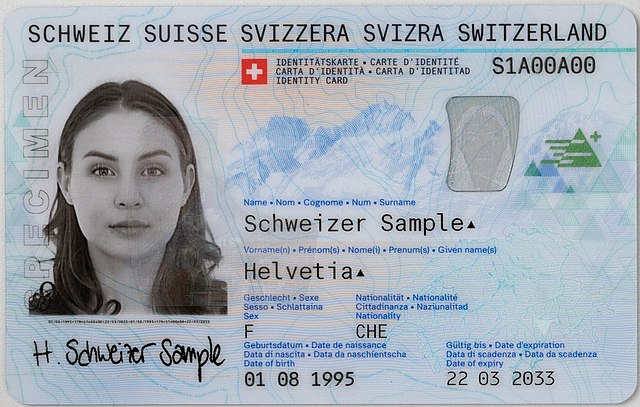
\includegraphics[width=30mm]{./img/ID.jpg}}$$
		$$\overleftarrow{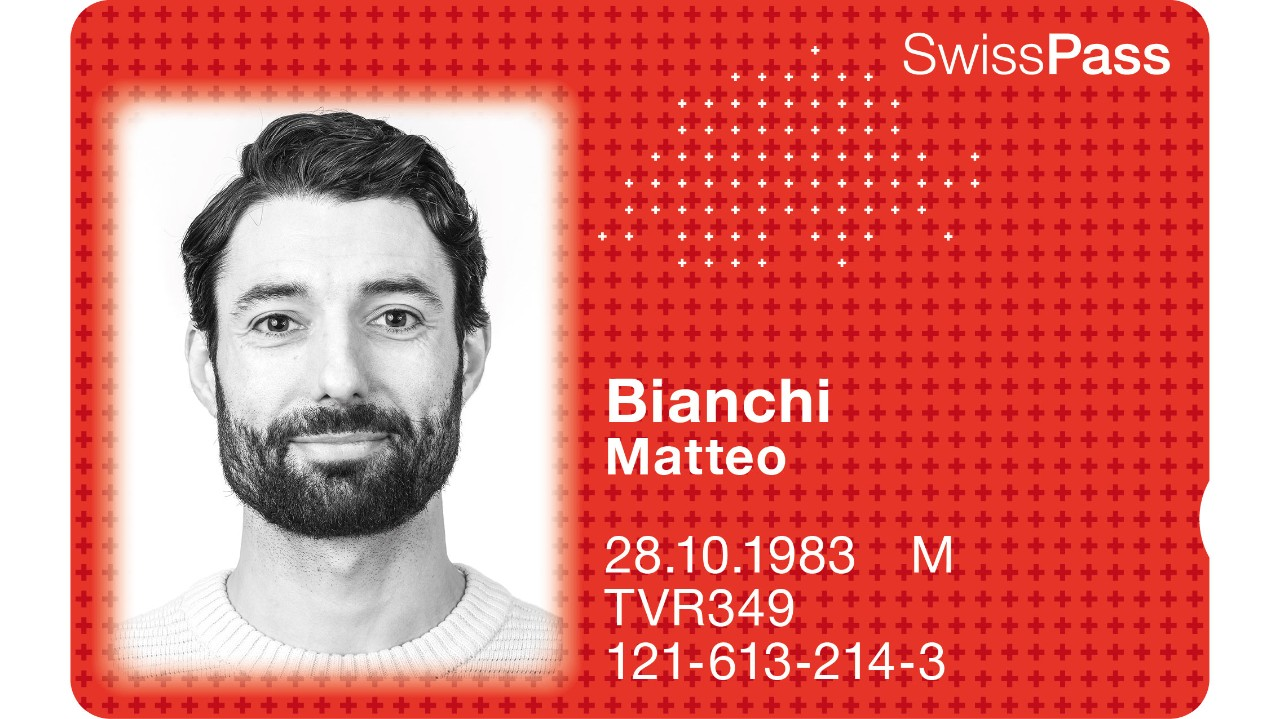
\includegraphics[width=30mm]{./img/Swisspass.jpeg}}$$
	\end{minipage}\hfill
	\begin{minipage}{0.28\textwidth}
		\textbf{SBB}\newline\newline
		
\begin{tikzpicture}
			\duck[tshirt, jacket=blue!50!black, tie=red]
		\end{tikzpicture}
	\end{minipage}
	\caption{Buying a train subscription}
	\label{fig:trainsub}
\end{figure}

Now you also need a mobile subscription. You go to your next Swiss Post office.

\begin{figure}[h]
	\begin{minipage}{0.28\textwidth}
		\textbf{Client}\newline\newline
		
\begin{tikzpicture}
			\duck[graduate]
		\end{tikzpicture}
	\end{minipage}\hfill

	\begin{minipage}{0.28\textwidth}
		$$\underrightarrow{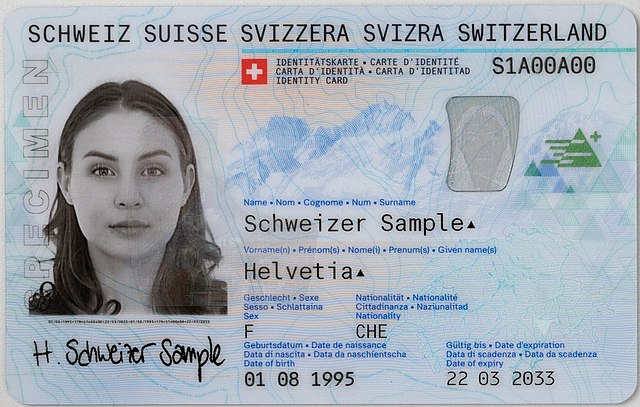
\includegraphics[width=30mm]{./img/ID.jpg}}$$
		$$\overleftarrow{\includegraphics[width=30mm]{example-image-duck}}$$
	\end{minipage}\hfill

	\begin{minipage}{0.28\textwidth}
		\textbf{Swiss Post}\newline\newline
		
\begin{tikzpicture}
			\duck[tshirt, jacket=yellow!50!orange, tie=black]
		\end{tikzpicture}
	\end{minipage}
	
	\caption{Buying a mobile subscription}
	\label{fig:mobilesub}
\end{figure}

Here, the employee makes the same checks as the SBB employee to see if you are who you say you are.
And again, by handing out your ID, you lose the ability to selectively disclose information about yourself.

\begin{figure}
	\includegraphics[width=30mm]{example-image-duck}
\end{figure}

Now lets say but verifiers collude. As they have the same information about you, they link it back to you and create a profile about.
In \autoref{chap:bbsex} we will see how we can use BBS to restore unlinkability and more.

\chapter{Extensions with BBS}
\label{chap:bbsex}
In this chapter we will analyze what VCs are and how they need to be manipulated to be signed by BBS.

\section{BBS with VC's}
The BBS signatures and proofs as well as the messages need to be transported somehow.
For this Thesis we chose Verifiable credentials \cite{verifiable-credentials} as the representation of these attributes.
But what are VC's? \newline
Verifiable credentials are JSON-LD data models, designed to represent different types of digital credentials.
The Idea, is to be able to translate physical credentials, like an ID or a driver's license, into the digital world.\\
In this Thesis we will only look at a small part of the standard, just enough that we can use it together with BBS.
We will also use VPs, or Verifiable Presentations. This is how VCs are called that are passed between a Holder and a verifier.
All VC concepts described can also be applied to VPs, so VP and VC can be used interchangeably.

\subsection{Used VC concepts}
In this section we will define which VC concepts are used in this thesis.

\subsubsection{@context}
The \textbf{@context} attribute is used to map human-friendly ids like \textit{type} to an url.
These urls then help the system understand what the content of the VC is.
The value of the \textbf{@context} attribute is an ordered list, where the first entry must be \textit{\url{https://www.w3.org/ns/credentials/v2}}.\\
We will also use the context \textit{\url{https://w3id.org/security/data-integrity/v2}} to signify that the content of the VC is protected.
Lastly we use a custom context, which describes the content in the credentialSubject.\newpage

Our custom context looks like this:
\begin{lstlisting}[language=json,firstnumber=1,caption={Example custom context},captionpos=b]
{
    "@context":{
        "first_name": "https://schema.org/givenName",
        "last_name": "https://schema.org/familyName"
    }
}
\end{lstlisting}

The complete \textbf{@context} which we will use in our example, where the different contexts are represented by urls, looks like this:
\begin{lstlisting}[language=json,firstnumber=1,caption={Example context},captionpos=b]
{
	"@context": [
		"https://www.w3.org/ns/credentials/v2",
		"https://w3id.org/security/data-integrity/v2",
		"https://raw.githubusercontent.com/RockstaYT/BA_Thesis_BBS_Signatures/docs/context/example_1.jsonld"
	],
}
\end{lstlisting}

\subsubsection{Id}
We are able to add an \textbf{Id} to the VC. This Id can be used to identify a VC or to use it for revocation purposes.\\
There are two places where an \textbf{Id} can be added:
\begin{enumerate}
	\item In the root of the VC, such that the whole VC can be identified
	\item Inside an object of a credentialSubject (see chapter \ref{subsub:credentialsubject}) to identify a specific subject
\end{enumerate}

These Ids must be \textit{urls} and be either a UUID, a DID or an HTTP URL.

\subsubsection{type}

The \textbf{type} defines what the VC is. 
It is a set containing either urls to the description of the VC or be an ID that can be mapped through \textbf{@context}.
If we use the standard mapped IDs, the type set must either include \textit{VerifiableCredential} or \textit{VerifiablePresentation}.
If we want, we can also add a more specific type, in which we define more information about the VC.\\
In this thesis we won't use any custom types.

\subsubsection{credentialSubject}
\label{subsub:credentialsubject}
The \textbf{credentialSubject} contains a set of objects, which each contain one or more statements about the subject of the credential.\\
In our first example we only have one object with two statements about the subject, namely \textit{first\_name} and \textit{last\_name}.\\
Such a credentialSubject may look like this:
\begin{lstlisting}[language=json,firstnumber=1,caption={Example credentialSubject},captionpos=b]
{
	"credentialSubject":{
		"first_name": "John",
		"last_name": "Doe"
	}
}
\end{lstlisting}

\subsubsection{proof}
The \textbf{proof} inside a VC guaranties its Integrity. But it can also do much more.
In this thesis the proof will either contain a BBS Signature, which signed the VC and with that guaranties its integrity, or it contains a BBS proof, which enables selective disclosure between and unlinkability between holder and verifier.\\
The proof object contains following key-value pairs:
\begin{itemize}
	\item Type: The type of the proof. In this thesis we use the type \textit{DataIntegrityProof}
	\item CryptoSuite: Which cryptosuite was used. In this thesis we use \textit{bbs-2023}
	\item Created: A timestamp when the proof was created
	\item VerificationMethod: Which verification method is used. This value must be a string that maps to a URL. In this thesis we will use a URL to a public key
	\item ProofPurpose: For what purpose is the proof. In this thesis we will use \textit{assertionMethod}
	\item ProofValue: The proof value. In this thesis this is either a BBS Signature or Proof
\end{itemize}

\subsection{Prepare VCs for BBS and sign them}
\label{sub:preparevc}
Now that we know all the different concepts needed for this thesis, we can look into how to prepare the VC to be signed by the BBS signature scheme.\\
VCs are JSON-LD objects with multiple key-value pairs on different levels.\\
BBS can only sign statements, so somehow we need to transform the JSON-LD object into statements.\\
To achieve this we will use the \textit{Data Integrity BBS Cryptosuites draft}\cite{bbsvc}.\newpage

We will be using the following VC as an example.
\begin{lstlisting}[language=json,firstnumber=1,caption={Example VC},captionpos=b]
{
	"@context": [
		"https://www.w3.org/ns/credentials/v2",
		"https://w3id.org/security/data-integrity/v2",
		"https://raw.githubusercontent.com/RockstaYT/BA_Thesis_BBS_Signatures/docs/context/example_1.jsonld"
	],
	"type":  ["VerifiableCredential"],
	"credentialSubject":{
		"first_name": "John",
		"last_name": "Doe"
	}
}
\end{lstlisting}

We define following variables:\\
\textbf{vc}: The VC document\\
\textbf{hmac\_key}: A 32-bit random string, which is later used to initialize an HMAC\\
\textbf{verification\_method}: The url to the verification method\\
\textbf{mandatory\_attributes}: A set of attributes which are mandatory for the holder to disclose to the verifier. For this example we will set the \textit{first\_name} as mandatory. This may look like this: ["credentialSubject/first\_name"]\\

Now follow these steps to transform and sign the VC:
\begin{itemize}
	\item Set \textbf{proof\_config} and \textbf{canonical\_proof\_config} to the respective entry in the result of the algorithm described in chapter 1.2 in the Analysis Document, with the inputs \textbf{vc.@context} and \textbf{verification\_method}
	\item Set \textbf{transformed\_document} to the result of the algorithm described in chapter 1.3 in the Analysis Document, with the inputs \textbf{vc}, \textbf{mandatory\_attributes} and \textbf{hmac\_key}.
	\item Set \textbf{hash\_data} to the result of the algorithm described in chapter 1.4 in the Analysis Document, with the inputs \textbf{canonical\_proof\_config}, \textbf{mandatory\_attributes} and \textbf{transformed\_document}
	\item Set \textbf{base\_proof} to the result of the algorithm described in chapter 1.5 in the Analysis Document, with the inputs \textbf{hash\_data} and \textbf{mandatory\_attributes}.
	\item Set \textbf{signed\_vc} to the result of the algorithm described in chapter chapter 1.6 in the Analysis Document, with the inputs \textbf{vc}, \textbf{proof\_config} and \textbf{base\_proof}.
\end{itemize}

And with that \textbf{signed\_vc} is a valid signed VC, that can be used to generate a derived VP with selective disclosure and unlinkable proofs.\\

This VC may look like this:

\begin{lstlisting}[language=json,firstnumber=1,caption={Signed VC},captionpos=b]
{
	"@context": [
		"https://www.w3.org/ns/credentials/v2"
	],
	"type": [
		"VerifiableCredential"
	],
	"credentialSubject": {
		"first_name": "John",
		"last_name": "Doe"
	},
	"proof": {
		"type": "DataIntegrityProof",
		"cryptosuite": "bbs-2023",
		"created": "2024-04-03T22:11:27.027Z",
		"verificationMethod": "did:key:zUC7D...",
		"proofPurpose": "assertionMethod",
		"proofValue": "u2V0ChdhAWFC2..."
	}
}
\end{lstlisting}

\subsection{Derive selective disclosure VPs}
As a holder of a secured VC, one would like to present that VC to a verifier.
For that we create a Verifiable Presentation (VP), which in turn is just a VC containing \textit{@context}, \textit{type} and the VC as \textit{verifiableCredential}.
We also want to use the selective disclosure provided by the BBS Signature Scheme, so that we don't need to disclose all the information contained in the VC.
We will use the same example as in chapter \ref{sub:preparevc}.\\
In that example we forced the disclosure of the \textit{last\_name}. We define that no more information should be revealed, meaning that the \textit{first\_name} will not be revealed to the verifier.\\

We define following variables:\\
\textbf{vc}: The VC, \textbf{not containing} the proof object\\
\textbf{base\_proof}: The proof object from the VC\\
\textbf{selective\_pointers}: A array containing pointers on what should be revealed. As already mentioned, in this example we will not reveal anything, so this variable is an empty array []\\
\textbf{ph}: The presentation header as a byte array. We will define it as an empty array [] for this example\\

To create the derived VP we call the algorithm in chapter 2.1 of the Analysis document, with the inputs \textbf{vc}, \textbf{base\_proof}, \textbf{selective\_pointers} and \textbf{ph}\\

This derived VP may look like this:
\begin{lstlisting}[language=json,firstnumber=1,caption={Derived VP},captionpos=b]
{
	"@context": [
		"https://www.w3.org/ns/credentials/v2",
		"https://w3id.org/security/data-integrity/v2",
		"https://raw.githubusercontent.com/RockstaYT/BA_Thesis_BBS_Signatures/docs/context/example_1.jsonld"
	],
	"type": [
		"VerifiableCredential"
	],
	"credentialSubject": {
		"first_name": "Joel"
	},
	"proof": {
		"type": "DataIntegrityProof",
		"cryptosuite": "bbs-2023",
		"created": "2024-04-17T23:41:58.089Z",
		"verificationMethod": "did:key:zUC7De...",
		"proofPurpose": "assertionMethod",
		"proofValue": "u2V0..."
	}
}
\end{lstlisting}

As you can see, the \textit{last\_name} is not shown as it is not being revealed.

\subsection{Verify derived VP}
\label{subsub:verifyvp}
A verifier has now received a selectively disclosed VP, which he would like to verify.\\

We define following variable:\\
\textbf{secured\_document}: This is the VP that was received from the holder\newpage

To verify the VP we follow these steps:
\begin{itemize}
	\item Set \textbf{unsecured\_document} to the copy of \textbf{secured\_document} but with the \textit{proof} value removed
	\item Set \textbf{proof\_config} to the copy of \textbf{secured\_document.proof} but with \textit{proofValue} value removed
	\item Set \textbf{proof} to the copy of \textbf{secured\_document.proof}
	\item Set \textbf{bbs\_proof}, \textbf{proof\_hash}, \textbf{non\_mandatory}, \textbf{mandatory\_hash}, \textbf{selective\_indexes}, \textbf{ph} and \textbf{feature\_option} to their respective entries in the result of the algorithm described in chapter 3.1 of the Analysis Document, with \textbf{unsecured\_document} and \textbf{proof} as the input
	\item Set \textbf{bbs\_header} to the concatenation of \textbf{proof\_hash} and \textbf{mandatory\_hash}
	\item Set \textbf{verify} to the result of the BBS Proof Verification algorithm defined in \textit{THE BBS Signature Scheme}\cite{bbs-signature-scheme} with the inputs \textbf{pk}, \textbf{bbs\_proof}, \textbf{bbs\_header}, \textbf{ph}
\end{itemize}

If \textbf{verify} is true, the verifier knows that the VP is valid and was not tampered with. 

\subsection{Security Considerations of VCs}
\label{subsec:vcseccons}
The combination of BBS and VC raises two security questions:
\begin{enumerate}
	\item If we want to use IDs to identify a revoked VC, we run into linkability problems
	\item The RDF canonicalization algorithm creates data leakage which leads to linkability
\end{enumerate}

\subsubsection{IDs in VCs}
While creating a VC, the issuer might add an ID to the VC to enable revocation.
A verifier can then check if the ID of the VC which was presented to them is in the revocation list of the issuer, and thus accept or reject the presentation.\\
But there is a big problem with this.
If the ID is just added to the VC and is revealed to multiple verifiers, they can link the presentations together based on the ID.
With that we would break the unlinkability provided by BBS.\\

To preserve the unlinkability between the presentations, the holder would need to be able to prove that the ID of the VC is not in the revocation list of the issuer.

As a solution to that problem, we can use a solution like ALLOSAUR\cite{allosaur}. 
With this solution a holder can prove to a verifier that his ID is not in the revocation list, without presenting a unique identifier.
In this thesis we will assume that the concept shown in ALLOSAUR works without compromising unlinkability.
We also won't look at how it works, as this would be out-of-scope for this thesis.

\subsubsection{RDF canonicalization algorithm}
In the algorithms described in the Analysis Document, we use RDF multiple times to transform the JSON-LD Document into statements.
Using this algorithm can lead to data leakage which in turn can lead to linkability.

Let's look at an example.
We will use the example given in chapter 6.1 of \textit{Data Integrity BBS Cryptosuites v1.0}\cite{bbsvc}:

\begin{lstlisting}[language=canon,firstnumber=1,caption={Example: Sails VC},captionpos=b]
{
	"@context": [
		"https://www.w3.org/ns/credentials/v2",
		{
		"@vocab": "https://windsurf.grotto-networking.com/selective#"
		}
	],
	"type": [
		"VerifiableCredential"
	],
	"credentialSubject": {
		"sails": [
		{
			"size": 5.5,
			"sailName": "Kihei",
			"year": 2023
		},
		{
			"size": 6.1,
			"sailName": "Lahaina",
			"year": 2023
		},
		{
			"size": 7.0,
			"sailName": "Lahaina",
			"year": 2020
		},
		{
			"size": 7.8,
			"sailName": "Lahaina",
			"year": 2023
		}
		]
	}
}
\end{lstlisting}

We use the RDF canonicalization algorithm and get these statements:

\begin{lstlisting}[language=canon,firstnumber=1,caption={Example: Sails VC as statements},captionpos=b]
[
	_:c14n0 <https://windsurf.grotto-networking.com/selective#sailName> "Lahaina" .
	_:c14n0 <https://windsurf.grotto-networking.com/selective#size> "7.8E0"^^<http://www.w3.org/2001/XMLSchema#double> .
	_:c14n0 <https://windsurf.grotto-networking.com/selective#year> "2023"^^<http://www.w3.org/2001/XMLSchema#integer> .
	_:c14n1 <http://www.w3.org/1999/02/22-rdf-syntax-ns#type> <https://www.w3.org/2018/credentials#VerifiableCredential> .
	_:c14n1 <https://www.w3.org/2018/credentials#credentialSubject> _:c14n4 .
	_:c14n2 <https://windsurf.grotto-networking.com/selective#sailName> "Lahaina" .
	_:c14n2 <https://windsurf.grotto-networking.com/selective#size> "7"^^<http://www.w3.org/2001/XMLSchema#integer> .
	_:c14n2 <https://windsurf.grotto-networking.com/selective#year> "2020"^^<http://www.w3.org/2001/XMLSchema#integer> .
	_:c14n3 <https://windsurf.grotto-networking.com/selective#sailName> "Kihei" .
	_:c14n3 <https://windsurf.grotto-networking.com/selective#size> "5.5E0"^^<http://www.w3.org/2001/XMLSchema#double> .
	_:c14n3 <https://windsurf.grotto-networking.com/selective#year> "2023"^^<http://www.w3.org/2001/XMLSchema#integer> .
	_:c14n4 <https://windsurf.grotto-networking.com/selective#sails> _:c14n0 .
	_:c14n4 <https://windsurf.grotto-networking.com/selective#sails> _:c14n2 .
	_:c14n4 <https://windsurf.grotto-networking.com/selective#sails> _:c14n3 .
	_:c14n4 <https://windsurf.grotto-networking.com/selective#sails> _:c14n5 .
	_:c14n5 <https://windsurf.grotto-networking.com/selective#sailName> "Lahaina" .
	_:c14n5 <https://windsurf.grotto-networking.com/selective#size> "6.1E0"^^<http://www.w3.org/2001/XMLSchema#double> .
	_:c14n5 <https://windsurf.grotto-networking.com/selective#year> "2023"^^<http://www.w3.org/2001/XMLSchema#integer> .
]
\end{lstlisting}

Now the data leakage problem arises in one specific case.
Let's say the holder only discloses information about the sails with the size 7.0 and 7.8, so the last two objects of the credentialSubject.\\
Now, the holder receives a new credential, where information about a sail, which has an entry before the disclosed sails (size 7.0 and 7.8), has been changed.
Let's say that the year for the size 6.0 sail has been updated to 2024.
When the RDF algorithm is now run again on the new VC, we get these statements:

\begin{lstlisting}[language=canon,firstnumber=1,caption={Example: Updated sails VC as statements},captionpos=b]
[
	_:c14n0 <https://windsurf.grotto-networking.com/selective#sailName> "Lahaina" .
	_:c14n0 <https://windsurf.grotto-networking.com/selective#size> "6.1E0"^^<http://www.w3.org/2001/XMLSchema#double> .
	_:c14n0 <https://windsurf.grotto-networking.com/selective#year> "2024"^^<http://www.w3.org/2001/XMLSchema#integer> .
	_:c14n1 <https://windsurf.grotto-networking.com/selective#sailName> "Lahaina" .
	_:c14n1 <https://windsurf.grotto-networking.com/selective#size> "7.8E0"^^<http://www.w3.org/2001/XMLSchema#double> .
	_:c14n1 <https://windsurf.grotto-networking.com/selective#year> "2023"^^<http://www.w3.org/2001/XMLSchema#integer> .
	_:c14n2 <http://www.w3.org/1999/02/22-rdf-syntax-ns#type> <https://www.w3.org/2018/credentials#VerifiableCredential> .
	_:c14n2 <https://www.w3.org/2018/credentials#credentialSubject> _:c14n5 .
	_:c14n3 <https://windsurf.grotto-networking.com/selective#sailName> "Lahaina" .
	_:c14n3 <https://windsurf.grotto-networking.com/selective#size> "7"^^<http://www.w3.org/2001/XMLSchema#integer> .
	_:c14n3 <https://windsurf.grotto-networking.com/selective#year> "2020"^^<http://www.w3.org/2001/XMLSchema#integer> .
	_:c14n4 <https://windsurf.grotto-networking.com/selective#sailName> "Kihei" .
	_:c14n4 <https://windsurf.grotto-networking.com/selective#size> "5.5E0"^^<http://www.w3.org/2001/XMLSchema#double> .
	_:c14n4 <https://windsurf.grotto-networking.com/selective#year> "2023"^^<http://www.w3.org/2001/XMLSchema#integer> .
	_:c14n5 <https://windsurf.grotto-networking.com/selective#sails> _:c14n0 .
	_:c14n5 <https://windsurf.grotto-networking.com/selective#sails> _:c14n1 .
	_:c14n5 <https://windsurf.grotto-networking.com/selective#sails> _:c14n3 .
	_:c14n5 <https://windsurf.grotto-networking.com/selective#sails> _:c14n4 .
]
\end{lstlisting}

You can see how the ordering is different, and how the blank nodes (\_:c14nx) where assigned differently.
Even if we didn't disclose any information about the two smaller sails before and after the VC update, a verifier could easily deduce that the content of the VC has changed, which is leaking data and depending on the size of the VC or what was already revealed, this can even lead to linkability.

There is an easy solution to this problem.
As an input to the RDF algorithm we need to pass a function, which takes the canonical label and replaces them with another value.
If we now add a HMAC (using SHA-256) to this function, we can randomize how the canonical label values are replaced each time a VC is created.

Note: It was suggested that the possibility to use KMAC with SHA3-256 should be added to the specification. This was declined by the working group on the basis that SHA-256 is more common.

\section{BBS with Pseudonyms}
\label{chap:Pseudonyms}

\section{BBS with Link Secrets}
\label{chap:linksecrets}

\section{BBS with Blind Signatures}
\label{chap:blindsignatures}




\appendix


\chapter{First appendix Chapter}



\bibliographystyle{plain}
\bibliography{refs}

\end{document}
